\documentclass[twoside]{book}

% Packages required by doxygen
\usepackage{calc}
\usepackage{doxygen}
\usepackage{graphicx}
\usepackage[utf8]{inputenc}
\usepackage{makeidx}
\usepackage{multicol}
\usepackage{multirow}
\usepackage{textcomp}
\usepackage[table]{xcolor}

% NLS support packages
\usepackage{polski}
\usepackage[T1]{fontenc}

% Font selection
\usepackage[T1]{fontenc}
\usepackage{mathptmx}
\usepackage[scaled=.90]{helvet}
\usepackage{courier}
\usepackage{amssymb}
\usepackage{sectsty}
\renewcommand{\familydefault}{\sfdefault}
\allsectionsfont{%
  \fontseries{bc}\selectfont%
  \color{darkgray}%
}
\renewcommand{\DoxyLabelFont}{%
  \fontseries{bc}\selectfont%
  \color{darkgray}%
}

% Page & text layout
\usepackage{geometry}
\geometry{%
  a4paper,%
  top=2.5cm,%
  bottom=2.5cm,%
  left=2.5cm,%
  right=2.5cm%
}
\tolerance=750
\hfuzz=15pt
\hbadness=750
\setlength{\emergencystretch}{15pt}
\setlength{\parindent}{0cm}
\setlength{\parskip}{0.2cm}
\makeatletter
\renewcommand{\paragraph}{%
  \@startsection{paragraph}{4}{0ex}{-1.0ex}{1.0ex}{%
    \normalfont\normalsize\bfseries\SS@parafont%
  }%
}
\renewcommand{\subparagraph}{%
  \@startsection{subparagraph}{5}{0ex}{-1.0ex}{1.0ex}{%
    \normalfont\normalsize\bfseries\SS@subparafont%
  }%
}
\makeatother

% Headers & footers
\usepackage{fancyhdr}
\pagestyle{fancyplain}
\fancyhead[LE]{\fancyplain{}{\bfseries\thepage}}
\fancyhead[CE]{\fancyplain{}{}}
\fancyhead[RE]{\fancyplain{}{\bfseries\leftmark}}
\fancyhead[LO]{\fancyplain{}{\bfseries\rightmark}}
\fancyhead[CO]{\fancyplain{}{}}
\fancyhead[RO]{\fancyplain{}{\bfseries\thepage}}
\fancyfoot[LE]{\fancyplain{}{}}
\fancyfoot[CE]{\fancyplain{}{}}
\fancyfoot[RE]{\fancyplain{}{\bfseries\scriptsize Wygenerowano Cz, 12 mar 2015 02\-:38\-:41 dla L\-A\-B1 programem Doxygen }}
\fancyfoot[LO]{\fancyplain{}{\bfseries\scriptsize Wygenerowano Cz, 12 mar 2015 02\-:38\-:41 dla L\-A\-B1 programem Doxygen }}
\fancyfoot[CO]{\fancyplain{}{}}
\fancyfoot[RO]{\fancyplain{}{}}
\renewcommand{\footrulewidth}{0.4pt}
\renewcommand{\chaptermark}[1]{%
  \markboth{#1}{}%
}
\renewcommand{\sectionmark}[1]{%
  \markright{\thesection\ #1}%
}

% Indices & bibliography
\usepackage{natbib}
\usepackage[titles]{tocloft}
\setcounter{tocdepth}{3}
\setcounter{secnumdepth}{5}
\makeindex

% Custom commands
\newcommand{\clearemptydoublepage}{%
  \newpage{\pagestyle{empty}\cleardoublepage}%
}


%===== C O N T E N T S =====

\begin{document}

% Titlepage & ToC
\pagenumbering{roman}
\begin{titlepage}
\vspace*{7cm}
\begin{center}%
{\Large L\-A\-B1 \\[1ex]\large 0.\-1 }\\
\vspace*{1cm}
{\large Wygenerowano przez Doxygen 1.8.6}\\
\vspace*{0.5cm}
{\small Cz, 12 mar 2015 02:38:41}\\
\end{center}
\end{titlepage}
\clearemptydoublepage
\tableofcontents
\clearemptydoublepage
\pagenumbering{arabic}

%--- Begin generated contents ---
\chapter{Indeks klas}
\section{Lista klas}
Tutaj znajdują się klasy, struktury, unie i interfejsy wraz z ich krótkimi opisami\-:\begin{DoxyCompactList}
\item\contentsline{section}{{\bf Benchmark$<$ T $>$} }{\pageref{class_benchmark}}{}
\item\contentsline{section}{{\bf Kolejka$<$ T $>$} \\*Klasa \doxyref{Kolejka}{str.}{class_kolejka} sluzy do wykonywania podstawowych operacji na Kolejce\-: dodaj,odejmij element. Przechowuje informacje o ilosci wszysktich elementow }{\pageref{class_kolejka}}{}
\item\contentsline{section}{{\bf List$<$ T $>$} \\*Klasa \doxyref{List}{str.}{class_list} sluzy do wykonywania podstawowych operacji na Liscie\-: dodaj,odejmij element. Przechowuje informacje o ilosci wszysktich elementow }{\pageref{class_list}}{}
\item\contentsline{section}{{\bf Node$<$ T $>$} }{\pageref{struct_node}}{}
\item\contentsline{section}{{\bf Node\-L$<$ T $>$} }{\pageref{struct_node_l}}{}
\item\contentsline{section}{{\bf Node\-T$<$ Klucz, T $>$} }{\pageref{class_node_t}}{}
\item\contentsline{section}{{\bf Stack$<$ T $>$} }{\pageref{class_stack}}{}
\item\contentsline{section}{{\bf Tablica\-Asocjacyjna} }{\pageref{class_tablica_asocjacyjna}}{}
\end{DoxyCompactList}

\chapter{Indeks plików}
\section{Lista plików}
Tutaj znajduje się lista wszystkich plików z ich krótkimi opisami\-:\begin{DoxyCompactList}
\item\contentsline{section}{{\bf Benchmark.\-hh} \\*Klasa \doxyref{Benchmark}{str.}{class_benchmark} sluzy do przechowywania wynikow zlozonosci obliczeniowej i danych wejsciowych,generowania liczb rozkladu Gaussowego }{\pageref{_benchmark_8hh}}{}
\item\contentsline{section}{{\bf Kolejka.\-hh} \\*Struktura przechowujaca wartosc wezla i wskaznik na nastepny element typu \doxyref{Node}{str.}{struct_node} }{\pageref{_kolejka_8hh}}{}
\item\contentsline{section}{{\bf Lista.\-hh} \\*Struktura przechowujaca wartosc wezla i wskaznik na nastepny element typu \doxyref{Node}{str.}{struct_node} }{\pageref{_lista_8hh}}{}
\item\contentsline{section}{{\bf main.\-cpp} }{\pageref{main_8cpp}}{}
\item\contentsline{section}{{\bf main3.\-cpp} }{\pageref{main3_8cpp}}{}
\item\contentsline{section}{{\bf Operacje\-Na\-Plikach.\-hh} }{\pageref{_operacje_na_plikach_8hh}}{}
\item\contentsline{section}{{\bf Sortowanie.\-cpp} }{\pageref{_sortowanie_8cpp}}{}
\item\contentsline{section}{{\bf Sortowanie.\-hh} }{\pageref{_sortowanie_8hh}}{}
\item\contentsline{section}{{\bf Stack.\-hh} \\*Klasa \doxyref{Stack}{str.}{class_stack} sluzy do przechowywania, dodawania,zdejmowania kolejnych elementow stosu }{\pageref{_stack_8hh}}{}
\item\contentsline{section}{{\bf Struktury.\-hh} }{\pageref{_struktury_8hh}}{}
\item\contentsline{section}{{\bf Zapisz\-Stos\-Kolejka\-Lista.\-cpp} }{\pageref{_zapisz_stos_kolejka_lista_8cpp}}{}
\item\contentsline{section}{{\bf Zapisz\-Stos\-Kolejka\-Lista.\-hh} }{\pageref{_zapisz_stos_kolejka_lista_8hh}}{}
\end{DoxyCompactList}

\chapter{Dokumentacja klas}
\section{Dokumentacja klasy Benchmark}
\label{class_benchmark}\index{Benchmark@{Benchmark}}


{\ttfamily \#include $<$Benchmark.\-hh$>$}

\subsection*{Metody publiczne}
\begin{DoxyCompactItemize}
\item 
{\bf Benchmark} ()
\item 
{\bf Benchmark} (int roz, unsigned long int max)
\item 
{\bf $\sim$\-Benchmark} ()
\item 
void {\bf Ustal\-Rozmiar\-Tablicy\-Zlozonosci\-Obliczeniowej} (int roz)
\item 
std\-::ostream \& {\bf Generuj\-Liczby\-Zmiennoprzecinkowe} (long int {\bf rozmiar}, std\-::ostream \&strum)
\item 
void {\bf Transformacja\-Boxa\-\_\-\-Mullera} (float a[$\,$])
\item 
void {\bf Stworz\-Liczby\-Odniesienia} (int p[$\,$], int ile)
\item 
void {\bf Testuj} (int Ilosc\-Powtorzen, int Max\-Ilosc\-Danych, void($\ast$wsk\-\_\-fun)(double $\ast$, int))
\item 
std\-::ostream \& {\bf Zapisz\-Wyniki\-Zlozonosci\-Obliczeniowej} (std\-::ostream \&Strm, int roz)
\end{DoxyCompactItemize}
\subsection*{Atrybuty publiczne}
\begin{DoxyCompactItemize}
\item 
long int $\ast$$\ast$ {\bf Zlozonosc\-Obliczeniowa}
\item 
double $\ast$ {\bf Liczby\-Gaussowe}
\item 
unsigned long int {\bf Ilosc\-Danych}
\item 
int {\bf rozmiar}
\end{DoxyCompactItemize}


\subsection{Opis szczegółowy}


Definicja w linii 10 pliku Benchmark.\-hh.



\subsection{Dokumentacja konstruktora i destruktora}
\index{Benchmark@{Benchmark}!Benchmark@{Benchmark}}
\index{Benchmark@{Benchmark}!Benchmark@{Benchmark}}
\subsubsection[{Benchmark}]{\setlength{\rightskip}{0pt plus 5cm}Benchmark\-::\-Benchmark (
\begin{DoxyParamCaption}
{}
\end{DoxyParamCaption}
)}\label{class_benchmark_acfca497989836a688d44477802e822d8}
brief Konstruktor bezparametryczny

Konstruktor bezparametryczny klasy \doxyref{Benchmark}{str.}{class_benchmark} Ustawia wszystkie zmienne i wskazniki na wartosc 0 

Definicja w linii 35 pliku Benchmark.\-cpp.

\index{Benchmark@{Benchmark}!Benchmark@{Benchmark}}
\index{Benchmark@{Benchmark}!Benchmark@{Benchmark}}
\subsubsection[{Benchmark}]{\setlength{\rightskip}{0pt plus 5cm}Benchmark\-::\-Benchmark (
\begin{DoxyParamCaption}
\item[{int}]{roz, }
\item[{unsigned long int}]{max}
\end{DoxyParamCaption}
)}\label{class_benchmark_ad4255005c516cdbffa2f66e6339dd675}
brief Konstruktor z 2 argumentami int, unsigned long int

Konstruktor parametryczny klasy \doxyref{Benchmark}{str.}{class_benchmark} 
\begin{DoxyParams}[1]{Parametry}
\mbox{\tt in}  & {\em roz} & -\/ typ int, rozmiar tablicy Zlozonosc\-Obliczeniowa, \\
\hline
\mbox{\tt in}  & {\em max-\/} & unsigned long int, ilosc liczb zmiennoprzecinkowych tablicy Liczby\-Gaussowe \\
\hline
\end{DoxyParams}


Definicja w linii 21 pliku Benchmark.\-cpp.

\index{Benchmark@{Benchmark}!$\sim$\-Benchmark@{$\sim$\-Benchmark}}
\index{$\sim$\-Benchmark@{$\sim$\-Benchmark}!Benchmark@{Benchmark}}
\subsubsection[{$\sim$\-Benchmark}]{\setlength{\rightskip}{0pt plus 5cm}Benchmark\-::$\sim$\-Benchmark (
\begin{DoxyParamCaption}
{}
\end{DoxyParamCaption}
)}\label{class_benchmark_a20476e07f09e2b20ed3e9a7f13a570e6}
brief destruktor klasy \doxyref{Benchmark}{str.}{class_benchmark} 

Definicja w linii 43 pliku Benchmark.\-cpp.



\subsection{Dokumentacja funkcji składowych}
\index{Benchmark@{Benchmark}!Generuj\-Liczby\-Zmiennoprzecinkowe@{Generuj\-Liczby\-Zmiennoprzecinkowe}}
\index{Generuj\-Liczby\-Zmiennoprzecinkowe@{Generuj\-Liczby\-Zmiennoprzecinkowe}!Benchmark@{Benchmark}}
\subsubsection[{Generuj\-Liczby\-Zmiennoprzecinkowe}]{\setlength{\rightskip}{0pt plus 5cm}ostream \& Benchmark\-::\-Generuj\-Liczby\-Zmiennoprzecinkowe (
\begin{DoxyParamCaption}
\item[{long int}]{rozmiar, }
\item[{std\-::ostream \&}]{strum}
\end{DoxyParamCaption}
)}\label{class_benchmark_ad6be812f42f324e7a50ecb75d607040e}
brief Funkcja generuje liczby typu double z rozkladu Gaussa

Funkcja generuje liczby typu float o rozkladzie Gaussa i zapisuje do strumienia 
\begin{DoxyParams}[1]{Parametry}
\mbox{\tt in}  & {\em rozmiar} & -\/ long int, ilosc wygenerowanych elementow \\
\hline
\mbox{\tt in}  & {\em \&strum} & -\/ referencja do strumienia wyjsciowego \\
\hline
\end{DoxyParams}
\begin{DoxyReturn}{Zwraca}
Zwraca referencje do strumienia wyjsciowego 
\end{DoxyReturn}
\begin{DoxyPrecond}{Warunek wstępny}
Prawidlowe dzialanie funkcji Transformacja\-Boxa\-\_\-\-Mullera 
\end{DoxyPrecond}


Definicja w linii 108 pliku Benchmark.\-cpp.

\index{Benchmark@{Benchmark}!Stworz\-Liczby\-Odniesienia@{Stworz\-Liczby\-Odniesienia}}
\index{Stworz\-Liczby\-Odniesienia@{Stworz\-Liczby\-Odniesienia}!Benchmark@{Benchmark}}
\subsubsection[{Stworz\-Liczby\-Odniesienia}]{\setlength{\rightskip}{0pt plus 5cm}void Benchmark\-::\-Stworz\-Liczby\-Odniesienia (
\begin{DoxyParamCaption}
\item[{int}]{p[$\,$], }
\item[{int}]{ile}
\end{DoxyParamCaption}
)}\label{class_benchmark_a9f023bc3ca418b0a9bdc44e622091866}
brief Funkcja tworzy wygodne liczby odniesienia dla danej funkcji testowej o zadanym maximum

Funkcja tworzy liczby odniesienia, by lepiej dobrac ilosci danych do testu 
\begin{DoxyParams}[1]{Parametry}
\mbox{\tt in}  & {\em $<$em$>$p} & -\/ int, w tablicy ustalane sa argumenty liczb odniesienia \\
\hline
\mbox{\tt in}  & {\em ile-\/int,jak} & duzo ma zostac stworzonych liczb odniesienia \\
\hline
\end{DoxyParams}
\begin{DoxyPrecond}{Warunek wstępny}
Ilosc liczb odniesienia musi byc podzielna przez 4 
\end{DoxyPrecond}


Definicja w linii 192 pliku Benchmark.\-cpp.

\index{Benchmark@{Benchmark}!Testuj@{Testuj}}
\index{Testuj@{Testuj}!Benchmark@{Benchmark}}
\subsubsection[{Testuj}]{\setlength{\rightskip}{0pt plus 5cm}void Benchmark\-::\-Testuj (
\begin{DoxyParamCaption}
\item[{int}]{Ilosc\-Powtorzen, }
\item[{int}]{Max\-Ilosc\-Danych, }
\item[{void($\ast$)(double $\ast$, int)}]{wsk\-\_\-fun}
\end{DoxyParamCaption}
)}\label{class_benchmark_a845e97251244e016fd76a211386ec9d6}
brief Funkcja mierzy czas trwania funkcji dla okreslonej ilosci danych

Funkcja sluzy do badania zlozonosci obliczeniowej danej funkcji 
\begin{DoxyParams}[1]{Parametry}
\mbox{\tt in}  & {\em Ilosc\-Powtorzen} & -\/ int, ile razy bedzie wykonany test \\
\hline
\mbox{\tt in}  & {\em Max\-Ilosc\-Danych} & -\/ int, maksymalna ilosc danych do testu \\
\hline
\mbox{\tt in}  & {\em wsk\-\_\-fun=} & wskaznik na funkcje testowana o arg\-:double$\ast$,int \\
\hline
\end{DoxyParams}
\begin{DoxyPrecond}{Warunek wstępny}
Poprawne dzialanie funkcji Stworz\-Liczby\-Odniesienia 
\end{DoxyPrecond}


Definicja w linii 149 pliku Benchmark.\-cpp.

\index{Benchmark@{Benchmark}!Transformacja\-Boxa\-\_\-\-Mullera@{Transformacja\-Boxa\-\_\-\-Mullera}}
\index{Transformacja\-Boxa\-\_\-\-Mullera@{Transformacja\-Boxa\-\_\-\-Mullera}!Benchmark@{Benchmark}}
\subsubsection[{Transformacja\-Boxa\-\_\-\-Mullera}]{\setlength{\rightskip}{0pt plus 5cm}void Benchmark\-::\-Transformacja\-Boxa\-\_\-\-Mullera (
\begin{DoxyParamCaption}
\item[{float}]{a[$\,$]}
\end{DoxyParamCaption}
)}\label{class_benchmark_a88cd04d5216ce593c83a2ace4d1fdca8}
brief Funkcja zamienia liczby float z rozkladu rownomiernego na Gaussowy

Funkcja zamienia liczby z rozkladu rownomiernego na rozklad Gaussa 
\begin{DoxyParams}[1]{Parametry}
\mbox{\tt in}  & {\em a\mbox{[}$\,$\mbox{]}} & -\/ typ float,wskaznik na tablice 2-\/elementowa \\
\hline
\end{DoxyParams}
\begin{DoxyPrecond}{Warunek wstępny}
2 liczby z rozkladu rownomiernego 
\end{DoxyPrecond}


Definicja w linii 134 pliku Benchmark.\-cpp.

\index{Benchmark@{Benchmark}!Ustal\-Rozmiar\-Tablicy\-Zlozonosci\-Obliczeniowej@{Ustal\-Rozmiar\-Tablicy\-Zlozonosci\-Obliczeniowej}}
\index{Ustal\-Rozmiar\-Tablicy\-Zlozonosci\-Obliczeniowej@{Ustal\-Rozmiar\-Tablicy\-Zlozonosci\-Obliczeniowej}!Benchmark@{Benchmark}}
\subsubsection[{Ustal\-Rozmiar\-Tablicy\-Zlozonosci\-Obliczeniowej}]{\setlength{\rightskip}{0pt plus 5cm}void Benchmark\-::\-Ustal\-Rozmiar\-Tablicy\-Zlozonosci\-Obliczeniowej (
\begin{DoxyParamCaption}
\item[{int}]{roz}
\end{DoxyParamCaption}
)}\label{class_benchmark_ae368ddb026799a351c48cca37f0d8101}
brief Ustalenie rozmiaru tablicy zlozonosci obliczeniowej

Funkcja ustala na nowo rozmiar tablicy Zlozonosc\-Obliczeniowa 
\begin{DoxyParams}[1]{Parametry}
\mbox{\tt in}  & {\em roz} & -\/ typ int, rozmiar tablicy Zlozonosc\-Obliczeniowa \\
\hline
\end{DoxyParams}
\begin{DoxyPrecond}{Warunek wstępny}
zmienna roz musi byc dodatnia 
\end{DoxyPrecond}


Definicja w linii 55 pliku Benchmark.\-cpp.

\index{Benchmark@{Benchmark}!Zapisz\-Wyniki\-Zlozonosci\-Obliczeniowej@{Zapisz\-Wyniki\-Zlozonosci\-Obliczeniowej}}
\index{Zapisz\-Wyniki\-Zlozonosci\-Obliczeniowej@{Zapisz\-Wyniki\-Zlozonosci\-Obliczeniowej}!Benchmark@{Benchmark}}
\subsubsection[{Zapisz\-Wyniki\-Zlozonosci\-Obliczeniowej}]{\setlength{\rightskip}{0pt plus 5cm}ostream \& Benchmark\-::\-Zapisz\-Wyniki\-Zlozonosci\-Obliczeniowej (
\begin{DoxyParamCaption}
\item[{std\-::ostream \&}]{Strm, }
\item[{int}]{roz}
\end{DoxyParamCaption}
)}\label{class_benchmark_aad2f9082804804036652cf9c51f7b503}
Funkcja sluzy do zapisania wynikow z tablicy Zlozonosc\-Obliczeniowa 
\begin{DoxyParams}[1]{Parametry}
\mbox{\tt in}  & {\em \&\-Strum} & -\/ referencja do strumienia wyjsciowego \\
\hline
\mbox{\tt in}  & {\em roz} & -\/ ilosc elementow w tablicy Zlozonosc\-Obliczniowa przez 2 \\
\hline
\end{DoxyParams}
\begin{DoxyReturn}{Zwraca}
Zwraca referencje do strumienia wyjsciowego 
\end{DoxyReturn}
\begin{DoxyPrecond}{Warunek wstępny}
Poprawnie wczytane wartosci tablicy Zlozonosc\-Obliczeniowa 
\end{DoxyPrecond}


Definicja w linii 211 pliku Benchmark.\-cpp.



\subsection{Dokumentacja atrybutów składowych}
\index{Benchmark@{Benchmark}!Ilosc\-Danych@{Ilosc\-Danych}}
\index{Ilosc\-Danych@{Ilosc\-Danych}!Benchmark@{Benchmark}}
\subsubsection[{Ilosc\-Danych}]{\setlength{\rightskip}{0pt plus 5cm}unsigned long int Benchmark\-::\-Ilosc\-Danych}\label{class_benchmark_af1a957a8d0a03f8ffe46254c2e70fb00}
brief ilosc liczb z rozkladu Gaussa 

Definicja w linii 24 pliku Benchmark.\-hh.

\index{Benchmark@{Benchmark}!Liczby\-Gaussowe@{Liczby\-Gaussowe}}
\index{Liczby\-Gaussowe@{Liczby\-Gaussowe}!Benchmark@{Benchmark}}
\subsubsection[{Liczby\-Gaussowe}]{\setlength{\rightskip}{0pt plus 5cm}double$\ast$ Benchmark\-::\-Liczby\-Gaussowe}\label{class_benchmark_a724da083f84249bfa2fd30526b249aab}
brief wskaznik na tablice przechowujaca elementy z rozkladu gaussa 

Definicja w linii 20 pliku Benchmark.\-hh.

\index{Benchmark@{Benchmark}!rozmiar@{rozmiar}}
\index{rozmiar@{rozmiar}!Benchmark@{Benchmark}}
\subsubsection[{rozmiar}]{\setlength{\rightskip}{0pt plus 5cm}int Benchmark\-::rozmiar}\label{class_benchmark_af99294c0704a176c5fda8dc47e2eb1e5}
brief ilosc liczb zlozonosci obliczeniowej 

Definicja w linii 28 pliku Benchmark.\-hh.

\index{Benchmark@{Benchmark}!Zlozonosc\-Obliczeniowa@{Zlozonosc\-Obliczeniowa}}
\index{Zlozonosc\-Obliczeniowa@{Zlozonosc\-Obliczeniowa}!Benchmark@{Benchmark}}
\subsubsection[{Zlozonosc\-Obliczeniowa}]{\setlength{\rightskip}{0pt plus 5cm}long int$\ast$$\ast$ Benchmark\-::\-Zlozonosc\-Obliczeniowa}\label{class_benchmark_ade239a0ce7d783ba10a387471e70a415}
brief wskaznik na tablice przechowujaca wartosci zlozonosci obliczeniowej(ilosc danych,czas) 

Definicja w linii 16 pliku Benchmark.\-hh.



Dokumentacja dla tej klasy została wygenerowana z plików\-:\begin{DoxyCompactItemize}
\item 
{\bf Benchmark.\-hh}\item 
{\bf Benchmark.\-cpp}\end{DoxyCompactItemize}

\chapter{Dokumentacja plików}
\section{Dokumentacja pliku Benchmark.\-cpp}
\label{_benchmark_8cpp}\index{Benchmark.\-cpp@{Benchmark.\-cpp}}
{\ttfamily \#include $<$iostream$>$}\\*
{\ttfamily \#include $<$chrono$>$}\\*
{\ttfamily \#include $<$cstdlib$>$}\\*
{\ttfamily \#include $<$ctime$>$}\\*
{\ttfamily \#include $<$cmath$>$}\\*
{\ttfamily \#include $<$fstream$>$}\\*
{\ttfamily \#include \char`\"{}Benchmark.\-hh\char`\"{}}\\*
\subsection*{Funkcje}
\begin{DoxyCompactItemize}
\item 
ostream \& {\bf operator$<$$<$} (ostream \&Strm, const {\bf Benchmark} \&ben)
\item 
istream \& {\bf operator$>$$>$} (istream \&Strm, {\bf Benchmark} \&ben)
\end{DoxyCompactItemize}


\subsection{Opis szczegółowy}
brief Definicja metod klasy \doxyref{Benchmark}{str.}{class_benchmark}

Zawiera definicje metod klasy \doxyref{Benchmark}{str.}{class_benchmark} 

Definicja w pliku {\bf Benchmark.\-cpp}.



\subsection{Dokumentacja funkcji}
\index{Benchmark.\-cpp@{Benchmark.\-cpp}!operator$<$$<$@{operator$<$$<$}}
\index{operator$<$$<$@{operator$<$$<$}!Benchmark.cpp@{Benchmark.\-cpp}}
\subsubsection[{operator$<$$<$}]{\setlength{\rightskip}{0pt plus 5cm}ostream\& operator$<$$<$ (
\begin{DoxyParamCaption}
\item[{ostream \&}]{Strm, }
\item[{const {\bf Benchmark} \&}]{ben}
\end{DoxyParamCaption}
)}\label{_benchmark_8cpp_aa820c985b6db3d4b3ca8752963c9f97d}
Funkcja operatorowa pozwala na wypisanie wszystkich liczb tablicy Liczby\-Gaussowe 
\begin{DoxyParams}[1]{Parametry}
\mbox{\tt in,out}  & {\em \&\-Strm} & -\/ referencja do strumienia wyjsciowego \\
\hline
\mbox{\tt in,out}  & {\em \&ben} & refencja do klasy typu \doxyref{Benchmark}{str.}{class_benchmark} \\
\hline
\end{DoxyParams}
\begin{DoxyReturn}{Zwraca}
Zwraca referencje do strumienia wyjsciowego 
\end{DoxyReturn}
\begin{DoxyPrecond}{Warunek wstępny}
Poprawne wczytanie liczb tablicy Liczby\-Gaussowe 
\end{DoxyPrecond}


Definicja w linii 75 pliku Benchmark.\-cpp.

\index{Benchmark.\-cpp@{Benchmark.\-cpp}!operator$>$$>$@{operator$>$$>$}}
\index{operator$>$$>$@{operator$>$$>$}!Benchmark.cpp@{Benchmark.\-cpp}}
\subsubsection[{operator$>$$>$}]{\setlength{\rightskip}{0pt plus 5cm}istream\& operator$>$$>$ (
\begin{DoxyParamCaption}
\item[{istream \&}]{Strm, }
\item[{{\bf Benchmark} \&}]{ben}
\end{DoxyParamCaption}
)}\label{_benchmark_8cpp_aebd792c01d9b28e675091ceee76aa5ba}
Funkcja operatorowa pozwala na wczytanie liczby typu double do tablicy Liczby\-Gaussowe 
\begin{DoxyParams}[1]{Parametry}
\mbox{\tt in,out}  & {\em \&\-Strm} & -\/ referencja do strumienia wejsciowego \\
\hline
\mbox{\tt in,out}  & {\em \&ben} & referencja do klasy typu \doxyref{Benchmark}{str.}{class_benchmark} \\
\hline
\end{DoxyParams}
\begin{DoxyReturn}{Zwraca}
Zwraca referencje do strumienia wejsciowego 
\end{DoxyReturn}
\begin{DoxyPrecond}{Warunek wstępny}
Liczba tylko typu double 
\end{DoxyPrecond}


Definicja w linii 92 pliku Benchmark.\-cpp.


\section{Dokumentacja pliku Benchmark.\-hh}
\label{_benchmark_8hh}\index{Benchmark.\-hh@{Benchmark.\-hh}}


Klasa \doxyref{Benchmark}{str.}{class_benchmark} sluzy do przechowywania wynikow zlozonosci obliczeniowej i danych wejsciowych,generowania liczb rozkladu Gaussowego.  


{\ttfamily \#include $<$iostream$>$}\\*
{\ttfamily \#include $<$chrono$>$}\\*
{\ttfamily \#include $<$cstdlib$>$}\\*
{\ttfamily \#include $<$ctime$>$}\\*
{\ttfamily \#include $<$cmath$>$}\\*
{\ttfamily \#include $<$fstream$>$}\\*
Wykres zależności załączania dla Benchmark.\-hh\-:
\nopagebreak
\begin{figure}[H]
\begin{center}
\leavevmode
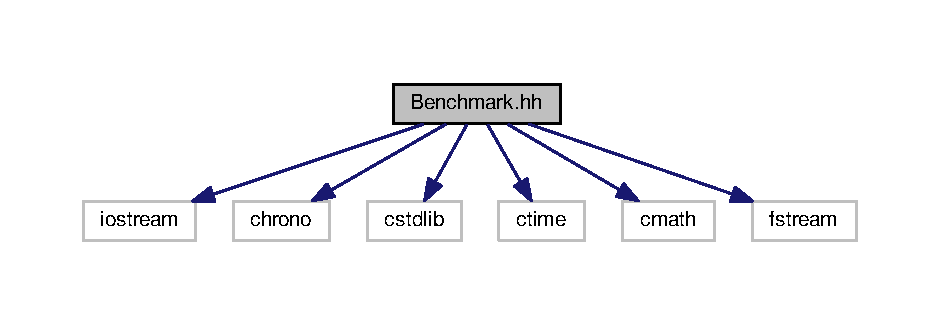
\includegraphics[width=350pt]{_benchmark_8hh__incl}
\end{center}
\end{figure}
Ten wykres pokazuje, które pliki bezpośrednio lub pośrednio załączają ten plik\-:
\nopagebreak
\begin{figure}[H]
\begin{center}
\leavevmode
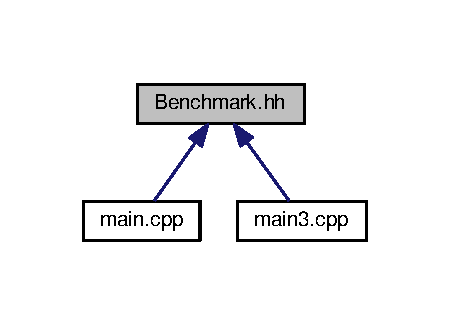
\includegraphics[width=216pt]{_benchmark_8hh__dep__incl}
\end{center}
\end{figure}
\subsection*{Komponenty}
\begin{DoxyCompactItemize}
\item 
class {\bf Benchmark$<$ T $>$}
\end{DoxyCompactItemize}
\subsection*{Funkcje}
\begin{DoxyCompactItemize}
\item 
{\footnotesize template$<$typename T $>$ }\\std\-::ostream \& {\bf operator$<$$<$} (std\-::ostream \&Strm, const {\bf Benchmark}$<$ T $>$ \&ben)
\item 
{\footnotesize template$<$typename T $>$ }\\std\-::istream \& {\bf operator$>$$>$} (std\-::istream \&Strm, {\bf Benchmark}$<$ T $>$ \&ben)
\end{DoxyCompactItemize}


\subsection{Dokumentacja funkcji}
\index{Benchmark.\-hh@{Benchmark.\-hh}!operator$<$$<$@{operator$<$$<$}}
\index{operator$<$$<$@{operator$<$$<$}!Benchmark.hh@{Benchmark.\-hh}}
\subsubsection[{operator$<$$<$}]{\setlength{\rightskip}{0pt plus 5cm}template$<$typename T $>$ std\-::ostream\& operator$<$$<$ (
\begin{DoxyParamCaption}
\item[{std\-::ostream \&}]{Strm, }
\item[{const {\bf Benchmark}$<$ T $>$ \&}]{ben}
\end{DoxyParamCaption}
)}\label{_benchmark_8hh_a09165957505edd311379cffe3322da36}
Funkcja operatorowa pozwala na wypisanie wszystkich liczb tablicy Liczby\-Gaussowe 
\begin{DoxyParams}[1]{Parametry}
\mbox{\tt in,out}  & {\em \&\-Strm} & -\/ referencja do strumienia wyjsciowego \\
\hline
\mbox{\tt in,out}  & {\em \&ben} & refencja do klasy typu \doxyref{Benchmark}{str.}{class_benchmark} \\
\hline
\end{DoxyParams}
\begin{DoxyReturn}{Zwraca}
Zwraca referencje do strumienia wyjsciowego 
\end{DoxyReturn}
\begin{DoxyPrecond}{Warunek wstępny}
Poprawne wczytanie liczb tablicy Liczby\-Gaussowe 
\end{DoxyPrecond}


Definicja w linii 140 pliku Benchmark.\-hh.

\index{Benchmark.\-hh@{Benchmark.\-hh}!operator$>$$>$@{operator$>$$>$}}
\index{operator$>$$>$@{operator$>$$>$}!Benchmark.hh@{Benchmark.\-hh}}
\subsubsection[{operator$>$$>$}]{\setlength{\rightskip}{0pt plus 5cm}template$<$typename T $>$ std\-::istream\& operator$>$$>$ (
\begin{DoxyParamCaption}
\item[{std\-::istream \&}]{Strm, }
\item[{{\bf Benchmark}$<$ T $>$ \&}]{ben}
\end{DoxyParamCaption}
)}\label{_benchmark_8hh_a849f5a7f6bcdc2c75a3d6bc6367f792e}
Funkcja operatorowa pozwala na wczytanie liczby typu double do tablicy Liczby\-Gaussowe 
\begin{DoxyParams}[1]{Parametry}
\mbox{\tt in,out}  & {\em \&\-Strm} & -\/ referencja do strumienia wejsciowego \\
\hline
\mbox{\tt in,out}  & {\em \&ben} & referencja do klasy typu \doxyref{Benchmark}{str.}{class_benchmark} \\
\hline
\end{DoxyParams}
\begin{DoxyReturn}{Zwraca}
Zwraca referencje do strumienia wejsciowego 
\end{DoxyReturn}
\begin{DoxyPrecond}{Warunek wstępny}
Liczba tylko typu double 
\end{DoxyPrecond}


Definicja w linii 158 pliku Benchmark.\-hh.


\section{Dokumentacja pliku main.\-cpp}
\label{main_8cpp}\index{main.\-cpp@{main.\-cpp}}
{\ttfamily \#include $<$iostream$>$}\\*
{\ttfamily \#include $<$fstream$>$}\\*
{\ttfamily \#include $<$string$>$}\\*
{\ttfamily \#include $<$cstdlib$>$}\\*
{\ttfamily \#include \char`\"{}Benchmark.\-hh\char`\"{}}\\*
{\ttfamily \#include \char`\"{}Zapisz\-Stos\-Kolejka\-Lista.\-hh\char`\"{}}\\*
{\ttfamily \#include \char`\"{}Operacje\-Na\-Plikach.\-hh\char`\"{}}\\*
{\ttfamily \#include \char`\"{}Struktury.\-hh\char`\"{}}\\*
{\ttfamily \#include \char`\"{}Sortowanie.\-hh\char`\"{}}\\*
Wykres zależności załączania dla main.\-cpp\-:
\nopagebreak
\begin{figure}[H]
\begin{center}
\leavevmode
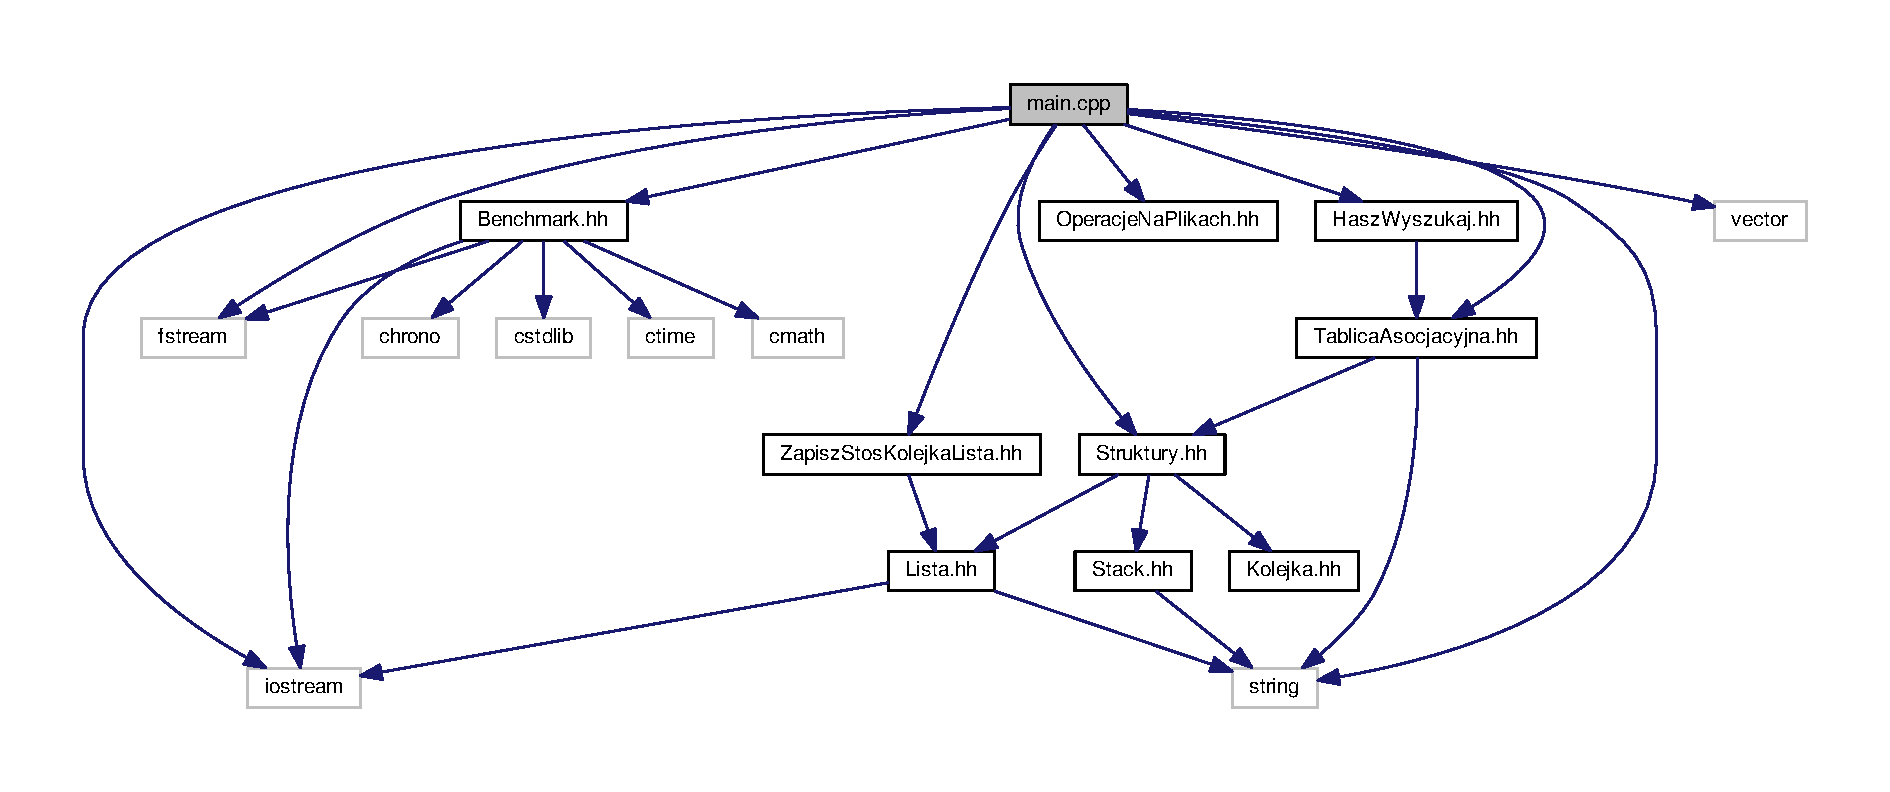
\includegraphics[width=350pt]{main_8cpp__incl}
\end{center}
\end{figure}
\subsection*{Funkcje}
\begin{DoxyCompactItemize}
\item 
int {\bf main} (int argc, char $\ast$argv[$\,$])
\end{DoxyCompactItemize}


\subsection{Dokumentacja funkcji}
\index{main.\-cpp@{main.\-cpp}!main@{main}}
\index{main@{main}!main.cpp@{main.\-cpp}}
\subsubsection[{main}]{\setlength{\rightskip}{0pt plus 5cm}int main (
\begin{DoxyParamCaption}
\item[{int}]{argc, }
\item[{char $\ast$}]{argv[$\,$]}
\end{DoxyParamCaption}
)}\label{main_8cpp_a0ddf1224851353fc92bfbff6f499fa97}


Definicja w linii 13 pliku main.\-cpp.



Oto graf wywołań dla tej funkcji\-:
\nopagebreak
\begin{figure}[H]
\begin{center}
\leavevmode
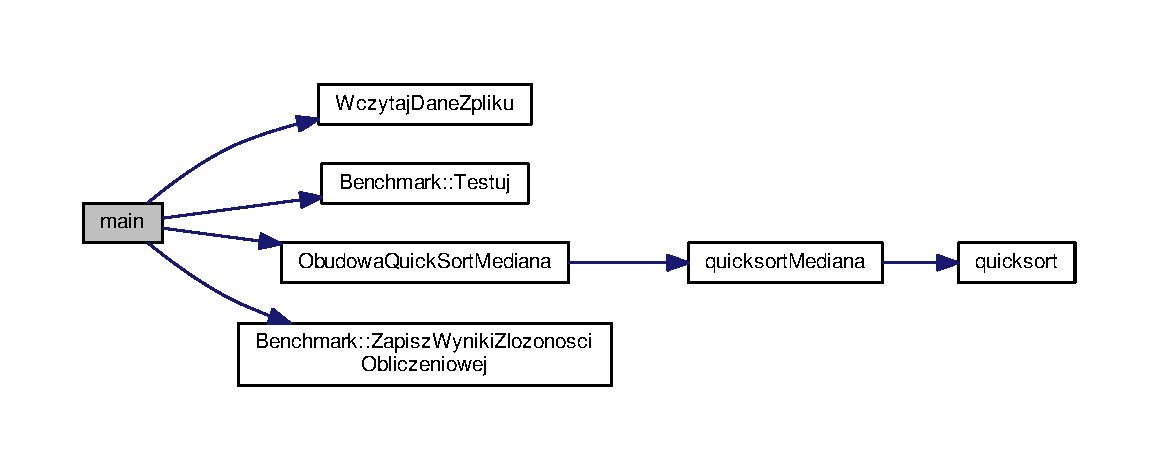
\includegraphics[width=350pt]{main_8cpp_a0ddf1224851353fc92bfbff6f499fa97_cgraph}
\end{center}
\end{figure}



%--- End generated contents ---

% Index
\newpage
\phantomsection
\addcontentsline{toc}{chapter}{Indeks}
\printindex

\end{document}
